\section{Exploitation}

\begin{figure}
  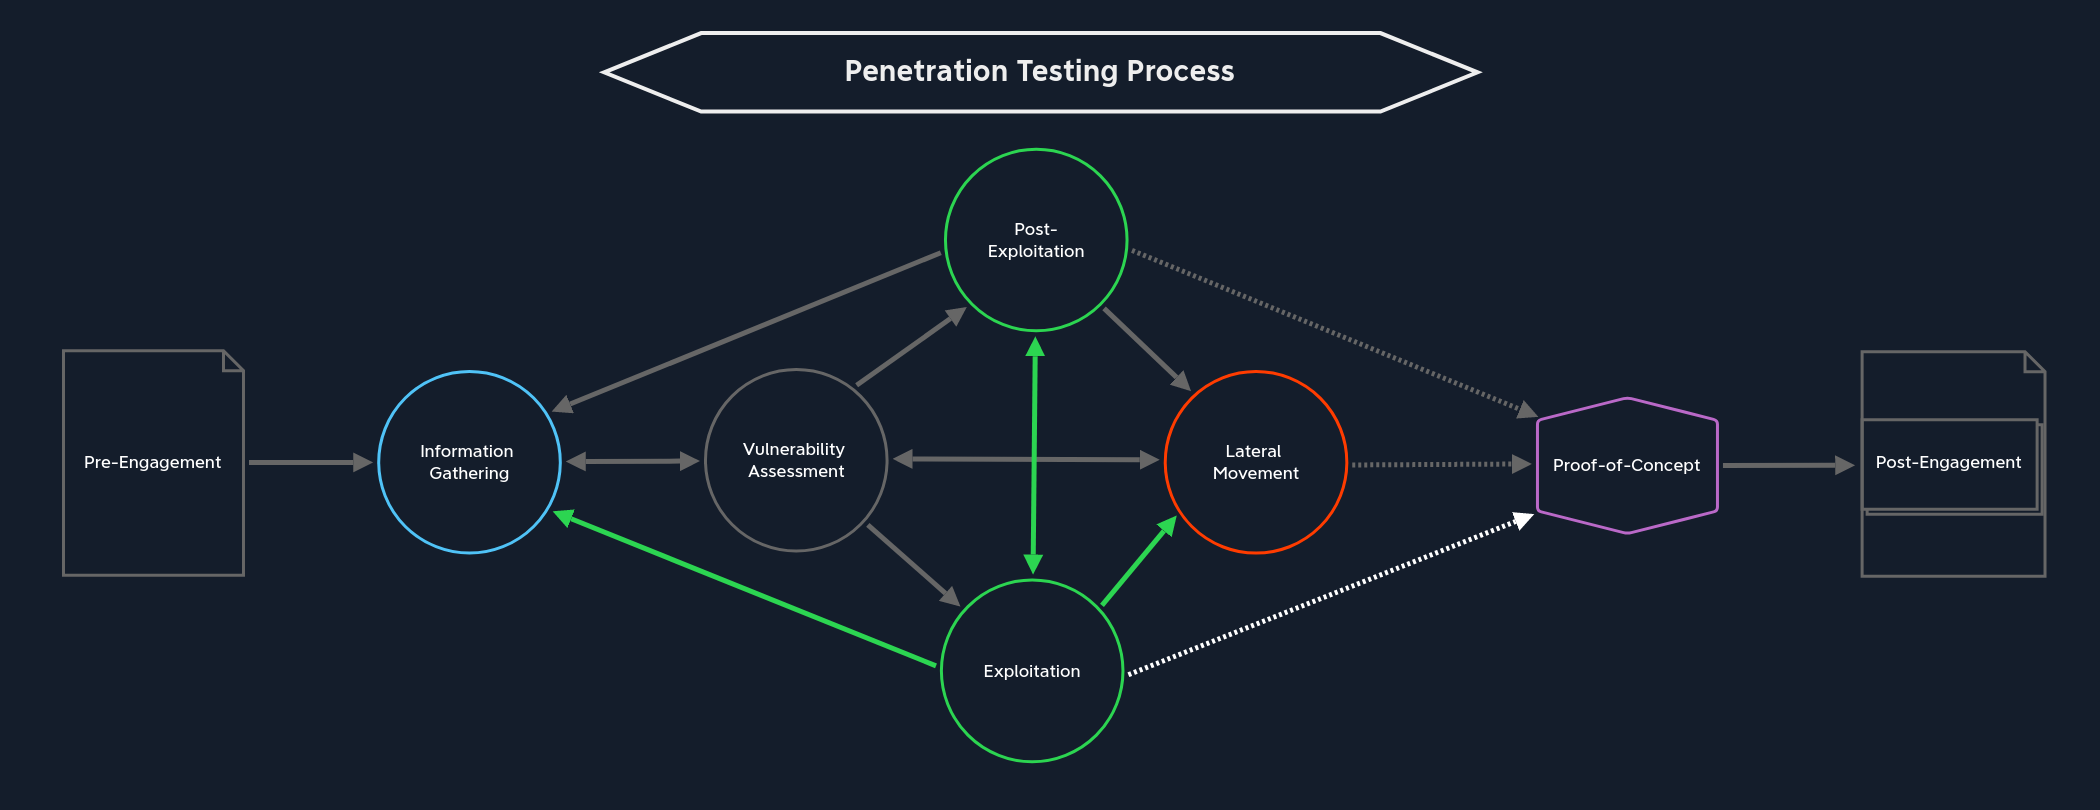
\includegraphics[width=\linewidth]{intro/process/images/exploit.png}
  \caption{Exploitation}
  \label{fig:pentest-process-exploit}
\end{figure}
During the Exploitation stage, we look for ways that these weaknesses can be
adapted to our use case to obtain the desired role (i.e., a foothold, escalated
privileges, etc.). If we want to get a reverse shell, we need to modify the PoC
to execute the code, so the target system connects back to us over (ideally) an
encrypted connection to an IP address we specify. Therefore, the preparation of
an exploit is mainly part of the Exploitation stage.

These stages should not be strictly separated from each other, as they are
closely connected. Nevertheless, it is still important to distinguish which
phase we are in and its purpose. Because later, with much more complex
processes and much more information, it is very easy to lose track of the steps
that have been taken, especially if the penetration test lasts several weeks
and covers a massive scope.

\subsection{Prioritization of Possible Attacks}
Once we have found one or two vulnerabilities during the Vulnerability
Assessment stage that we can apply to our target network/system, we can
prioritize those attacks. Which of those attacks we prioritize higher than the
others depends on the following factors:
\begin{itemize}
    \item  Probability of Success
    \item  Complexity
    \item  Probability of Damage
\end{itemize}

First, we need to assess the probability of successfully executing a particular
attack against the target. \href{https://nvd.nist.gov/vuln-metrics/cvss}{CVSS
Scoring} can help us here, using the
\href{https://nvd.nist.gov/vuln-metrics/cvss/v3-calculator}{NVD calculator}
better to calculate the specific attacks and their probability of success.

Complexity represents the effort of exploiting a specific vulnerability. This
is used to estimate how much time, effort, and research is required to execute
the attack on the system successfully. Our experience plays an important role
here because if we are to carry out an attack that we have never used before,
this will logically require much more research and effort since we must
understand the attack and the exploit structure in detail before applying it.

Estimating the probability of damage caused by the execution of an exploit
plays a critical role, as we must avoid any damage to the target systems.
Generally, we do not perform DoS attacks unless our client requires them.
Nevertheless, attacking the running services live with exploits that can cause
damage to the software or the operating system is something that we must avoid
at all times.


\subsection{Preparation for the Attack}
Sometimes we will run into a situation where we can't find high-quality, known
working PoC exploit code. Therefore, it may be necessary to reconstruct the
exploit locally on a VM representing our target host to figure out precisely
what needs to be adapted and changed. Once we have set up the system locally
and installed known components to mirror the target environment as closely as
possible (i.e., same version numbers for target services/applications), we can
start preparing the exploit by following the steps described in the exploit.
Then we test this on a locally hosted VM to ensure it works and does not damage
significantly. In other situations, we will encounter misconfigurations and
vulnerabilities that we see very often and know exactly which tool or exploit
to use and whether the exploit or technique is "safe" or can cause
instability.

If ever in doubt before running an attack, it's always best to check with our
client, providing them all necessary data so they can make an informed decision
on whether they would like us to attempt exploitation or just mark the finding
as an issue. If they opt for us not to proceed with exploitation, we can note
in the report that it was not confirmed actively but is likely an issue that
needs to be addressed. We have a certain amount of leeway during penetration
tests and should always use our best judgment if a particular attack seems too
risky or could potentially cause a disruption. When in doubt, communicate. Your
team lead/manager, the client, will almost certainly prefer extra communication
than run into a situation where they are trying to bring a system back online
after a failed exploit attempt.

Once we have successfully exploited a target and have initial access (and taken
clear notes for our reports and logged all activities in our activity log!),
we'll move on to the post-exploitation and lateral movement stages.
